The overarching aim of this project is to upgrade the lolly machine to a functioning state that accurately reflects the capabilities of Murdoch University ICSE students.
The project aims for the LMU2 are detailed as follows.

\subsection{Documentation}
    Along side thesis documentation, detailed design documents will need to be completed, documents include: a User guide, Schematics and IO test sheets.

\subsection{Mechanical Fixes}
    The machine needs to be fixed so that it can operate inline with its original intended use case. Additional functionality, in respect to mechanics,  will not be implemented. If any ideas regarding additional mechanical functionality come to fruition during the project they will be included in the final thesis document as future recommendations.
    
\subsection{Replace Embedded System}
    At this present time, a MC68HC11 based embedded system is responsible for the control, communication and operation of the lolly machine \cite{thesisJodie}. This system is comprised of three boards: the Interface Board, the I/O Board and the Processor Board.\\
    \begin{figure}[ht]
        \centering
        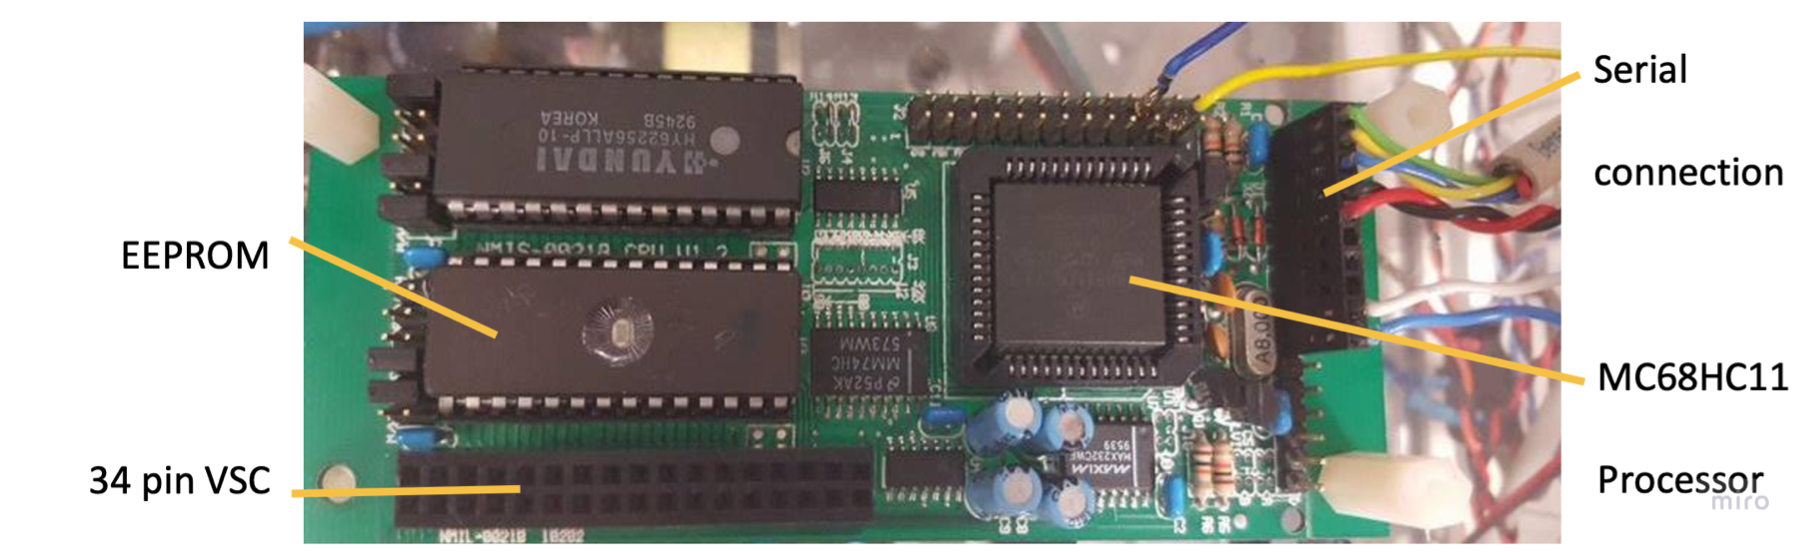
\includegraphics[scale = 0.2]{processorBoard.png}
        \caption{Processor board of lolly machine ~\cite{thesisJodie}.}
        \label{fig:processorBoard}
    \end{figure}
    Since the original build in 1996 by Graeme Cole and John Boulton \cite{computerControlGCole}, technological advancements have lead to smaller and more powerful micro-controllers and embedded systems \cite{mCHistory}. One of the key objectives of this project is to replace the three board MC68HC11-based embedded system by a HCS12-based embedded system comprised of a singular board, the Dragon12-Plus2 board, hereafter referred to as the Dragon board. 
    Although Dragon boards have ceased production due to a semi conductor shortage \cite{dragonBoardRevD}, Murdoch engineering stores have several as they were once part of the learning objectives in ENG319 (Real Time and Embedded Systems). An interface board connecting the Dragon board to the existing peripherals will need to be designed and manufactured prior to installation.\\
    \begin{figure}[ht]
        \centering
        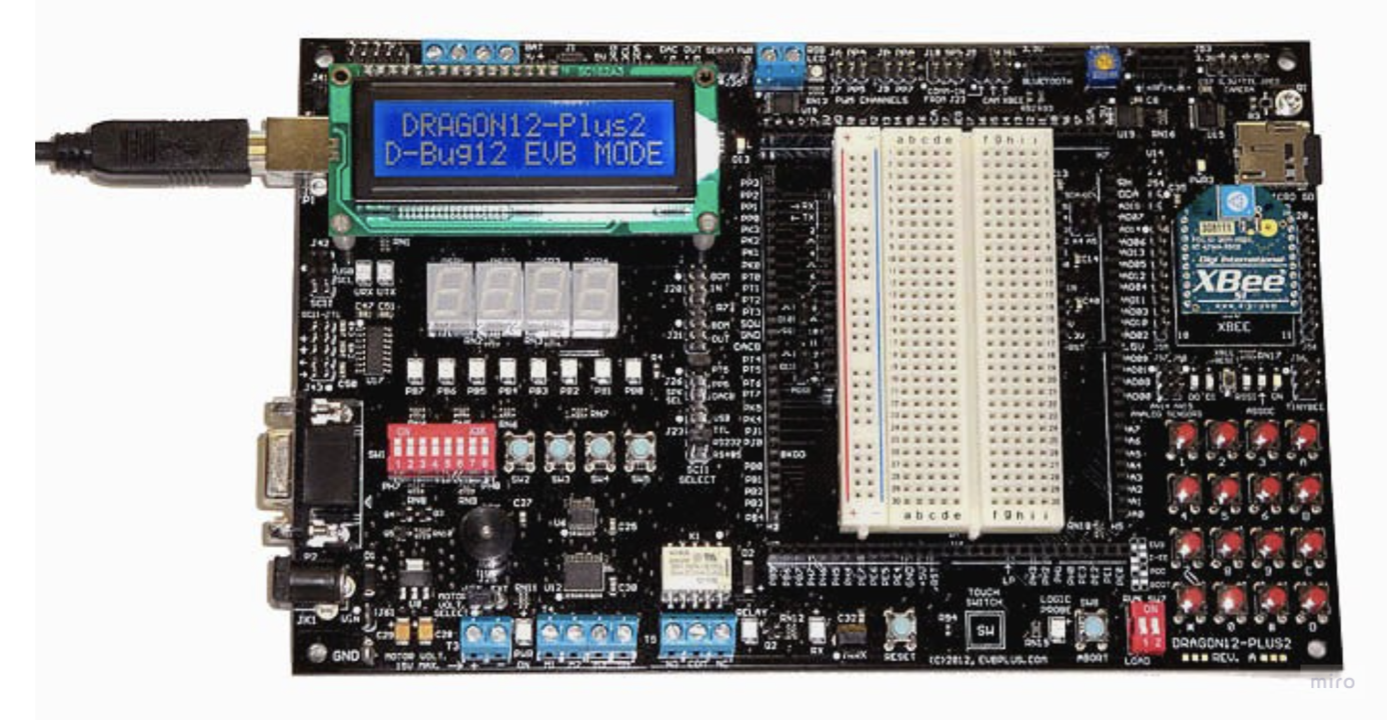
\includegraphics[scale = 0.2]{dragonBoard.png}
        \caption{Dragon12-Plus2 board to replace MC68HC11 based embedded system ~\cite{dragonBoard}.}
        \label{fig:dragonBoard}
    \end{figure}
    
\subsection{Pneumatic Valve Feedback}
    Sorting and dispensing is done through a series of pneumatic cylinders (linear non-rotating and rotating). Each cylinder is equip with two position feedback reed switches, these are currently not used. An addition to the program will include the use of cylinder position feedback. 
    
\subsection{Manual Mode}
    A manual mode will be added to the program allowing the user to manually read inputs and write to outputs. This added functionality will be helpful while testing IO and diagnosing problems. IO status will be presented on the LCD screen on the side of the unit while writing to outputs will be possible from the button pad adjacent to the LCD screen.
    
\subsection{LabVIEW HMI}
    The current user interface consists of: 
    \begin{itemize}
        \item Start and cancel buttons.
        \item Start, cancel and error LED indicators.
        \item 4 X Lolly colour increment buttons, one for each colour 
        \item 4 x Seven segment displays, one for each colour.
    \end{itemize}
    Alongside the existing user interface, a HMI will be developed in LabVIEW. The HMI will have the same functionality of the existing program but will provide a more intuitive interface in regard to operation and IO status. Subject to budget constraints, a windows based tablet will host the LabVIEW-Runtime executable, the tablet will be mounted on the side of the unit. A USB to RS232 protocol converter will provide connection between the tablet and the Dragon Board. During operation from the LabVIEW HMI the Dragon board will be in manual mode and respond to commands from the HMI via RS232.
    \\ \begin{figure}[ht]
        \centering
        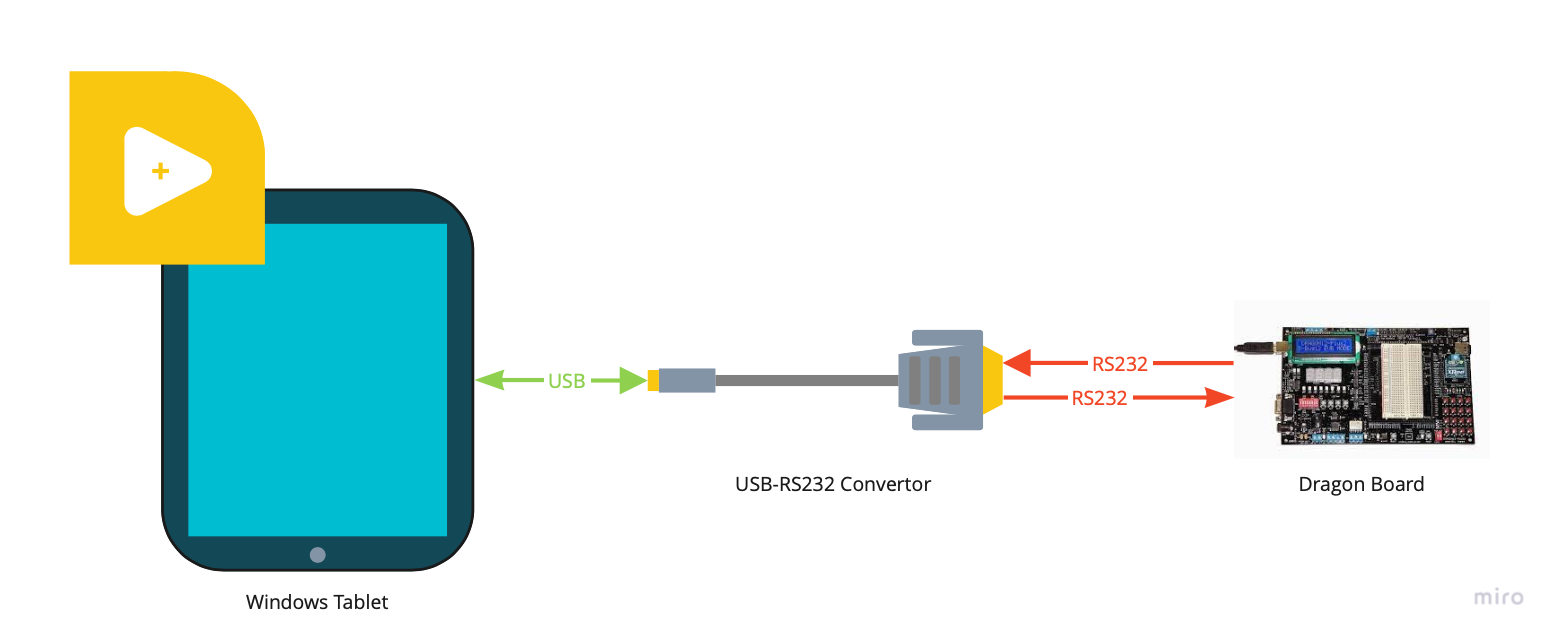
\includegraphics[scale = 0.2]{labHmiBlock.png}
        \caption{Block diagram of proposed LabVIEW HMI setup.}
        \label{fig:labHmiBlock}
    \end{figure}
    
\subsection{Web-Based HMI}
    The final objective for the LMU2 will be to design and build a web-based HMI. The HMI will be developed with Ignition Maker Edition and hosted on a Raspberry PI. The Raspberry PI will communicate through UDP with an ESP32. The ESP32 will then communicate with the Dragon board via RS232. While the system is being controlled via the web-based HMI the Dragon Board will be in manual mode and respond to commands from the ESP32 via RS232. An alternative option could be to host Ignition Maker on the LabVIEW HMI tablet.
    \\ \begin{figure}[ht]
        \centering
        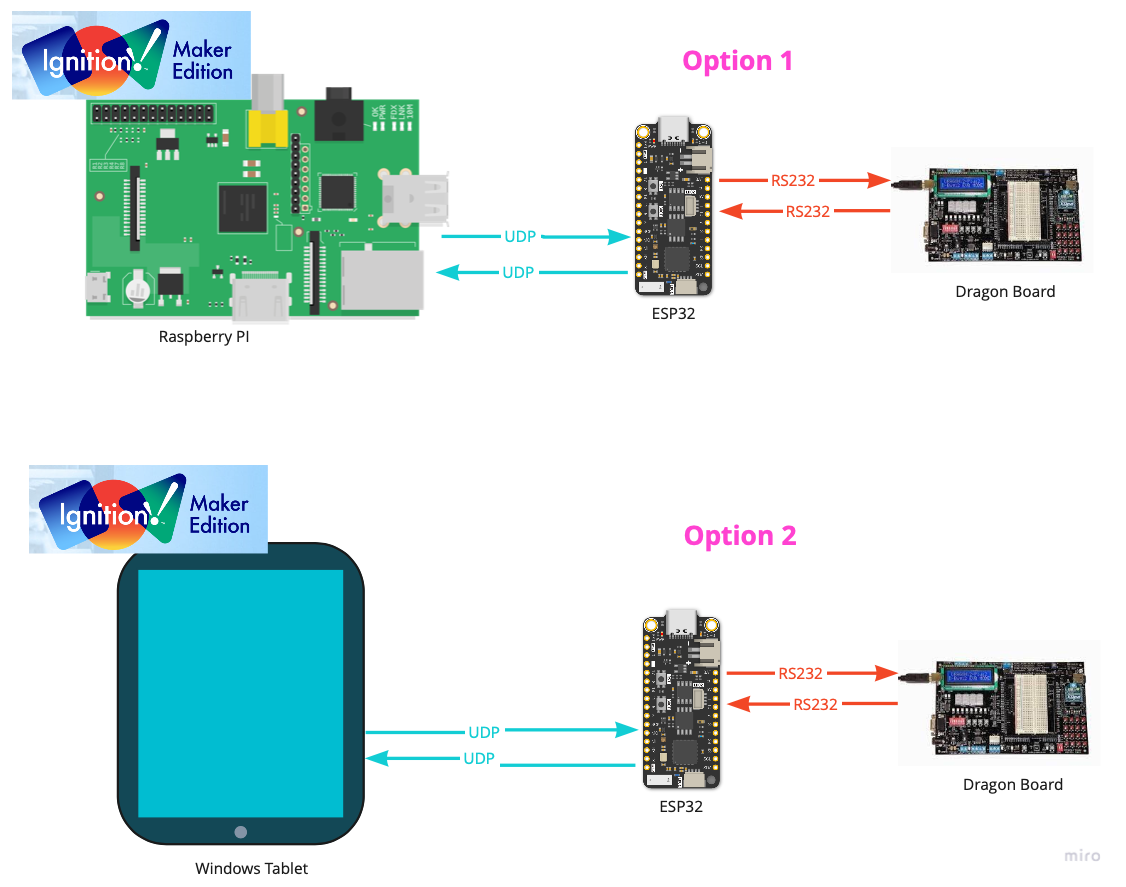
\includegraphics[scale = 0.2]{webHmiBlock.png}
        \caption{Block diagram of proposed web-based HMI setups.}
        \label{fig:webHmiBlock}
    \end{figure}
